% !LW recipe=pdflatex
% !TEX root = tvuontis.tex
%% This file is modified by Jussi Kangasharju and Pirjo Moen.
%% Earlier versions were made by Veli Mäkinen
%% from HY_fysiikka_LuKtemplate.tex authored by Roope Halonen ja
%% Tomi Vainio. Some text is also inherited from engl_malli.tex by
%% Kutvonen, Erkiö, Mäkelä, Verkamo, Kurhila, and Nykänen.
%% 
%% 
% STEP 1: Choose oneside or twoside
\documentclass[english,oneside,openany]{UH_DS_report}
%finnish,swedish
%
%\usepackage[utf8]{inputenc} 
% For UTF8 support. Use UTF8 when saving your file.
\usepackage{lmodern} % Font package 
\usepackage{textcomp} % Package for special symbols 
\usepackage[pdftex]{color, graphicx} % For pdf output and jpg/png graphics 
\usepackage[pdftex, plainpages=false]{hyperref} % For hyperlinks and pdf metadata 
\usepackage{fancyhdr} % For nicer page headers 
\usepackage{tikz} % For making vector graphics (hard to learn but powerful)
%\usepackage{wrapfig} % For nice text-wrapping figures (use at own discretion)
\usepackage{amsmath, amssymb} % For better math
%\usepackage[square]{natbib} % For bibliography
\usepackage[footnotesize,bf]{caption} % For more control over figure captions 
\usepackage{blindtext} 
\usepackage{titlesec}
\usepackage[titletoc]{appendix}
\usepackage{cleveref}

\onehalfspacing %line spacing
%\singlespacing 
%\doublespacing

%\fussy 
\sloppy % sloppy and fussy commands can be used to avoid overlong text lines

% STEP 2: 
% Set up all the information for the title page and the abstract form. 
% Replace parameters with your information.
\title{VMBC Report} 
\author{Tuomas Vuontisjarvi}

\date{\today}
\keywords{layout, summary, list of references} 
\depositeplace{}
\additionalinformation{}

% \classification{\protect{\ \\
%     \  General and reference $\rightarrow$ Document types $\rightarrow$ Surveys and overviews\  \\
%     \  Applied computing $\rightarrow$ Document management and text processing $\rightarrow$ Document management $\rightarrow$ Text editing\\
% }}

% If you want to quote someone special. You can comment this line and
% there will be nothing on the document.
%\quoting{Bachelor's degrees make pretty good placemats if you get them
%laminated.}{Jeph Jacques}

% OPTIONAL STEP: Set up properties and metadata for the pdf file that
% pdfLaTeX makes. But you don't really need to do this unless you want
% to.
\hypersetup{ 
	%bookmarks=true,         % show bookmarks bar first?
	unicode=true,           % to show non-Latin characters in Acrobat's bookmarks 
	pdftoolbar=true,        % show Acrobat's toolbar?
	pdfmenubar=true,        % show Acrobat's menu? 
	pdffitwindow=false,		% window fit to page when opened 
	pdfstartview={FitH},    % fits the width of the page to the window 
	pdftitle={},            % title
	pdfauthor={},           % author 
	pdfsubject={},          % subject of the document 
	pdfcreator={},          % creator of the document
	pdfproducer={pdfLaTeX}, % producer of the document
	pdfkeywords={something} {something else}, % list of keywords for
	pdfnewwindow=true,      % links in new window 
	colorlinks=true, 		% false: boxed links; true: colored links 
	linkcolor=black,        % color of internal links 
	citecolor=black,        % color of links to bibliography 
	filecolor=magenta,      % color of file links 
	urlcolor=cyan			% color of external links
}
          
\begin{document}

% Generate title page.
\maketitle

% STEP 3: Write your abstract (of course you really do this last). You
% can make several abstract pages (if you want it in different
% languages), but you should also then redefine some of the above
% parameters in the proper language as well, in between the abstract
% definitions.

\begin{abstract}
This report is about Variational Bayesian Monte Carlo (VBMC), a method for performing 
Bayesian inference with complex and computationally expensive black-box models. Key concepts
related to the VMBC are explained to provide clear a understanding of the background and the algorithm.
As the algorithm is also offered as a python package, usage examples are explored and used to explain 
VMBC even further.
\end{abstract}

% Place ToC
\mytableofcontents

\mynomenclature

% ----------------------------------------------------------------------
% STEP 4: Write the report. Your actual text starts here.
% You shouldn't mess with the code above the line except to change the
% parameters. Removing the abstract and ToC commands will mess up stuff.

\chapter{Introduction}
\label{chapter:intro}

According to Acerbi (2018), a significant problem with probabilistic models that have expensive,
black-box likelihoods is that the characteristics prevent the usage of standard techniques for 
Bayesian inference.

In order to address the problem of high computational cost, a novel sample efficient method 
has been introduced, called Variational Bayesian Monte Carlo (VMBC). 
Acerbi claims that the VMBC solves the previously costly problem by combining 
variational inference with Bayesian quadrature, solving model posteriors efficiently 
and with a relatively small amount of sampling\cite{acerbi2018}.

This report aims to explain the VMBC by exploring the key concepts behind it. 
Chapter three focuses on explaining all the relevant concepts and providing examples 
and on the way. The goal is to build a clear picture of the mathematical notions involved with the algorithm.

Chapter four will dive deeper into the workings of the VMBC
by using the python package pyVBMC provided by the author. 


\chapter{Key concepts and VMBC explained}
\label{chapter:structure}

% \begin{enumerate}
%   \renewcommand{\labelenumi}{\roman{enumi}.}
%   \item Black-box models
%   \item Bayesian inference
%   \item Approximate inference methods
%   \item Model posteriors
%   \item Gaussian process
%   \item Monte Carlo algorithms
% \end{enumerate}

The VMBC is used for complex and computationally expensive black-box models. 
Acerbi notes a few examples of such models, such as computational neuroscience, biology and 
big data models\cite{acerbi2018}\cite{acerbi2020}.
The algorithm is a novel approximate inference  method for learning about black-box models. A model is black-box model when there is no access to its inner processes. This means that the 
model can be viewed completely in terms of its inputs and outputs. 

One way of learning about the model is Bayesian inference, which is a method for computing posterior distribution
over parameters and the model evidence. However, since Bayesian inference is 
generally analytically intractable\cite{acerbi2018}, statistical approximate inference methods 
are often used. These methods include Markov Chain Monte Carlo algorithms and variational inference.

As Acerbi notes, existing methods of approximate inference, 
such as above examples, generally require knowledge about the 
model in order to produce approximate inference\cite{acerbi2018}. When a method requires more knowledge about the model
than just inputs and outputs, by definition it can't be applied to black-box models. Some methods
can bypass this requirement when given a very large number of model evaluations.

A computationally expensive black-box model is a model where evaluating the model is time consuming, 
which means that there generally isn't access to large number of model evaluations. Therefore the existing methods for approximate Bayesian inference are unfit for 
computationally expensive black-box models. Expensive model is defined as one evaluation taking 
one second or more per evaluation\cite{pyvmbc}

The VMBC produces a flexible approximate posterior distribution of the model parameters 
\cite{acerbi2018}. The posterior distribution is a joint probability distribution which describes 
how plausible each parameter is given the observed data. The posterior is expressed as $p(x \mid \mathcal{D})$,
where $\mathcal{D}$ is the dataset or the evidence and vector $x \in \mathbb{R}^D$ of the black-box model parameters.


The black-box model for the algorithm is expressed as $p(\mathcal{D} \mid x)$\cite{acerbi2018}.
From the point of view of the pyVBMC, a python package for performing VMBC model 
and posterior inference, the black-box model is provided as Python function, 
which calculates target log likelihood of the black-box model\cite{pyvmbc}. This means 
that from user point of view, the black-box model takes in a parameter vector representing the estimation
for the model parameters and calculates the likelihood of the data with the given parameters $\log p(\mathcal{D} \mid x)p(x)$.

A simple example of such log likelihood function could be a two value vector and a dataset of normally
distributed values with some specific mean and variance. 
The function then would solve the log likelihood of seeing that particular dataset with the proposed parameters,
which would stand for mean and variance.

The VMBC algorithm also computes the marginal likelihood, expressed as $p(\mathcal{D})$\cite{acerbi2018}. 
Fong and Holmes define marginal likelihood as a measure of 
model fit\cite{holmes}. They also note that when the model is correctly specified, 
the marginal likelihood provides a method for computing the posterior probability of the model
with the given data $\mathcal{D}$. Acerbi also calls marginal likelihood the model evidence\cite{acerbi2018}.

By definition it is the integral over the paramater space:

$$
p(\mathcal{D})=\int p(\mathcal{D}\mid x)p(x)dx
$$

Marginal likelihood is therefore a function, which means that is a mathematical 
description of the likelihoods over the whole paramater space. The VMBC algorithm uses 
marginal likelihood in the computation of the approximate posterior distribution\cite{acerbi2018}: 

$$p(x\mid\mathcal{D}) = \frac{p(\mathcal{D}\mid x)p(x)}{p(\mathcal{D})}$$

Thus, the computation of the algorithm has two components. Computing the marginal likelihood function and the 
approximate posterior distribution. $p(\mathcal{D}\mid x)$ is the likelihood of the model of interest and $p(x)$
is the prior over parameters.\cite{acerbi2018}

With the computational constraints, Acerbi suggests building a probabilistic model-based
approximation of the function of interest and propose Gaussian process for the build
process\cite{acerbi2018}.

According to Williams and Rasmussen, a Gaussian process is a generilaziation of the Gaussian
probability distribution\cite{gaussian}. They use the example of classifying handwritten symbols and 
a training set. The goal is not to just classify the existing data but move on to new unknown data 
and correctly classifying those. The task then is to transition from finite data to a function which
produces correct outputs for all possible inputs.
The problem is that there has to be some assumptions made about 
the function. A broad a definition could lead to overfitting, where the function describes 
the existing dataset very well but fails to produce correct outputs for new data. Or the 
definition could be too strict and fail to match to the target function.

One possible solution is to give prior probability to every possible function. But as Williams and Rasmussen note,
this leads to performing calculation on an infinite number of different possible functions. Instead, functions 
are considered as long vectors, where each vector value describes the output for the function $f(x)$ with the 
particular input. Even though these function vectors are infinetely long, the advantage of Gaussian process is that it 
gives the same answer for a finite number of points, whether you ignore all 
the infinite number of other points or not. And answers with different finite sets are 
consistent with each other.\cite{gaussian}

As example Williams and Rasmussen give a set of smooth curve functions with a lot of variation, where 
smoothness of a function is considered a prior. As
$x,y$ points are given and a requirement for a function to intersect with those points, a posterior distribution
of functions can be produced. The posterior functions still vary, but they all intersect in the given points.
Intuitively this means that each data point restricts the number of functions, because all the functions
that do not intersect given data points are concidered less likely. If different points are given, we have 
a different probability distribution for the functions, but the probable functions still include functions for
all other data points.\cite{gaussian}

\begin{figure}[h]
    \centering
    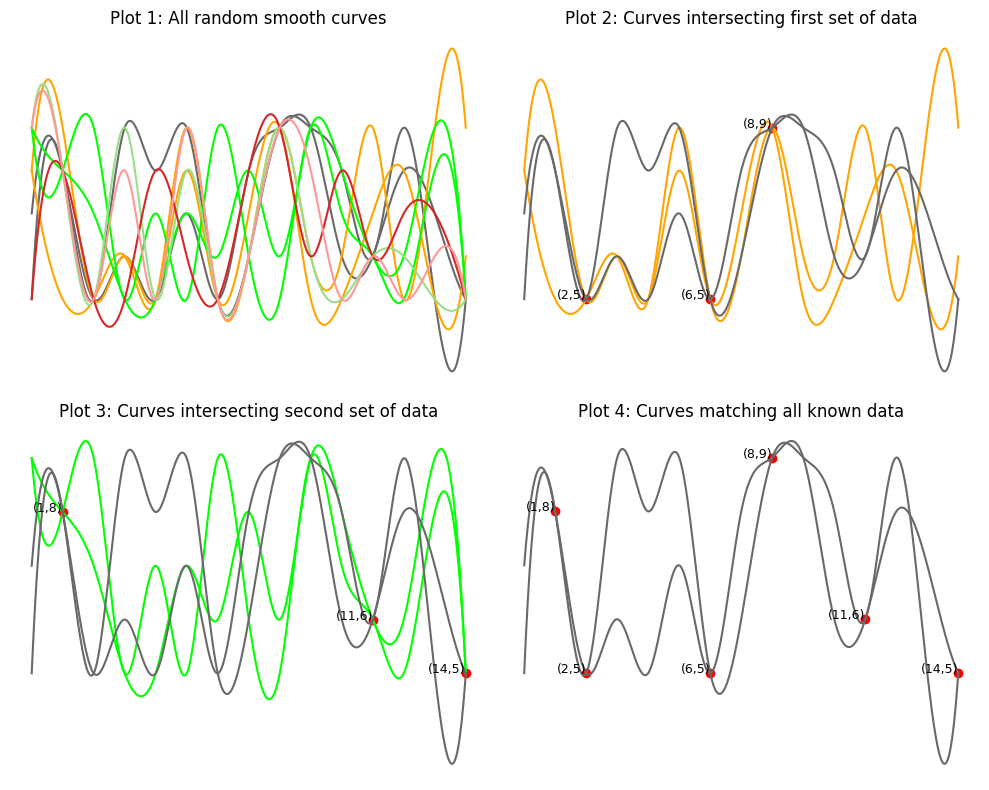
\includegraphics[width=0.75\textwidth]{plots.png}
    \caption{Smooth curves representing}
    \label{Fig:gp-curves}
\end{figure}

The \cref{Fig:gp-curves} provides a (flawed) illustration to build intuition. Plot 1 describe a large set of random smooth curves. Plot 2 shows
curves that match the first set of data, reducing the number of possible curves. Plot 3 shows curves matching
a different set of known data. Finally plot 4 shows the curves that match all of data. Notice that 
the curves in plot 4 can also be found in plot 2 and 3. This is a visual representation of how Gaussian process
gives consistent answers for different data - the set of possible curves gets restricted with data, but all
considered sets of data include the curves consistent with other sets of data. In actuality the GP doesn't 
deal with any particular function but a probability distribution of functions.

The VMBC uses Gaussian process based Bayesian quadrature to estimate the marginal likelihood\cite{acerbi2018}. 
According to Osborne \textit{et al.}, Bayesian quadrature provides a method for numerical integration with sample
efficiency. The method relies on a distribution of likelihood functions and a number of samples to provide
inferences about the distribution\cite{bayesian_quadrature}. The quadrature evaluates $f(x)$ at vector sample
points and performs analytic Gaussian process to infer about the value of the integral. In the VMBC, the 
quadrature provides mean and variance of the integral\cite{acerbi2018}.
The point of Bayesian quadrature then is to provide increasingly more accurate mean and variance of the
marginal likelihood, which was the integral: $p(\mathcal{D})=\int p(\mathcal{D}\mid x)p(x)dx$.

The VMBC algorithm is iterative and continues until a given budget of evaluations is depleted or when 
some termination criteria is reached. First step of the algorithm finds a set of samples that maximize given 
acquisition function, which are meant to guide optimal sampling. These sample points are then fed to the
given log likelihood function provided by the user\cite{acerbi2018}. In other words, VMBC produces excellent guesses for the $x$ in 
$p(\mathcal{D} \mid x)p(x)$ and then evaluates each guess for the black-box model.

Second step is to train a GP model based on the first step evaluations\cite{acerbi2018}. Here GP-based Bayesian quadrature 
is used to estimate the marginal likelihood: $p(\mathcal{D})=\int p(\mathcal{D}\mid x)p(x)dx$.
Third step is to update variational posterior approximation by optimizing the 
lower evidence bound\cite{acerbi2018}. In mathematical terms, this equates to solving the posterior
formula: $p(x\mid\mathcal{D}) = \frac{p(\mathcal{D}\mid x)p(x)}{p(\mathcal{D})}$, which is then used to guide 
the next iteration active sampling.

\chapter{pyVMBC examples}
\label{chapter:layout}

TODO

\chapter{Conclusions}
\label{chapter:conclusions}

TODO

% STEP 5: Uncomment the following lines and set your .bib file and
% desired bibliography style to make a bibliography with BibTeX.
% Alternatively you can use the thebibliography environment if you want
% to add all references by hand.
% 
\cleardoublepage %fixes the position of bibliography in bookmarks
\phantomsection

\renewcommand\bibname{References}
\addcontentsline{toc}{chapter}{\bibname} % This lines adds the bibliography to the ToC 
\bibliographystyle{abbrv} % numbering alphabetic order 
\bibliography{UH_DS_references}


\end{document}
